%% The CSAIL abstract book is a custom document class called 
%% "csailabstractbook".  It is based on the teTeX 1.0 distribution of LaTeX,
%% insofar as it uses a number of additional packages from teTeX for its
%% behind-the-scenes formatting. If you are using a different
%% distribution of LaTeX, it is possible that your distribution does not
%% have the necessary packages, in which case you will receive a missing 
%% package error when using the class file. You may wish to latex a copy 
%% of this file as-is to ensure that your configuration is correct.  

%% You should *not* include additional packages in preparing your
%% abstract.  The csailabstractbook class automatically includes the
%% standard "graphicx" package for inclusion of figures. An example of
%% its syntax is given in the text below, and more detailed documentation
%% can be found from the lab's latex page. Please use PDF files for your images.

%% Producing your abstract should be straightforward. Keeping all your
%% files in your working directory, run latex on the abstract file, bibtex
%% on the abstract file, and then latex on the abstract file twice.

\documentclass{csailabstractbook}

\begin{document}

%% The use of the sectioning commands, \abstitle and \absection, should 
%% be clear.  Try to follow the form of the sample text below, except
%% that your text should make a bit more sense.  It is ok to delete a 
%% section if it doesn't apply to your work.


\abstitle{An Integrated Development Environment for Streaming Systems}
         {Kimberly Kuo, Juan Reyes, Jasper Lin, Rodric Rabbah, and Saman Amarasinghe}

%% Please include an index entry for each author, keeping the names
%% consistent across abstracts. 
\index{Kuo, Kimberly}
\index{Reyes, Juan}
\index{Lin, Jasper}
\index{Rabbah, Rodric}
\index{Amarasinghe, Saman}

\absection{What}

StreamIt~\cite{streamitcc}  is a  high-level  architecture independent
language  for   modern  streaming   systems.   It  is   geared  toward
facilitating   the   rapid   implementation   of   complex   streaming
applications and  mitigating the need for  expert-level programmers on
the  critical path to  achieving high  performance.  Toward  this end,
StreamIt provides  a unified programming  model with a  single machine
abstraction,  irrespective of whether  the eventual  target is  a tiled
architecture, a cluster of workstations or a traditional uniprocessor.
Furthermore,  StreamIt  is  designed  to  promote  a  natural  textual
representation  of an application,  thereby improving  readability and
robustness, or  in other words, programmer productivity.   Our goal is
to leverage  the novel language  features in StreamIt to facilitate  practical and
large-scale  program development,  offering a  modular,  portable, and
malleable programming  paradigm.  Specifically, we  are developing the
StreamIt Development  Tool (SDT) which includes  graphical and textual
editors, as well as a  debugger that can interpret and visually convey
the dynamic behavior of a StreamIt application.

\absection{Why} 

Applications that  are structured around  some notion of  a ``stream''
are increasingly prevalent to common computing practices, and there is
evidence   that  streaming  media   applications  already   consume  a
substantial fraction  of the computation cycles  on consumer machines.
Furthermore, stream processing---of  voice and video data---is central
to a plethora of embedded systems, including hand-held computers, cell
phones,  and  DSPs. The  stream  abstraction  is  also fundamental  to
high-performance  systems such as  intelligent software  routers, cell
phone base stations, and HDTV editing consoles.

The  StreamIt  project  (see {\it www.cag.csail.mit.edu/streamit}  for  more
information) provides natural language constructs and high-performance
compiler technology for modern  stream programming. It is designed for
portability   across  machines   that  are   well-suited   for  stream
processing,  including  the  emerging class  of  communication-exposed
architectures such  as Raw~\cite{raw}.  Part  of the success of  the C
language  is  attributed to  its  portable  interface for  von-Neumann
machines: it abstracts away  the idiosyncratic differences between one
machine and  another, but exposes the common  and important properties
for achieving  high system  performance.  Similarly, StreamIt  aims to
provide a  portable language for next-generation  processors that have
replicated processing units  with software-exposed communication.  The
StreamIt  language  abstracts  away  the  granularity  of  a  parallel
machine, yet  exposes the regular communication  patterns and abundant
parallelism that are key to obtaining high performance.

Our goal is  to provide a StreamIt Development Tool  (SDT) as a robust
environment to promote the proliferation of StreamIt for practical and
large-scale program  design and  implementation. Toward this  end, our
work leverages  the StreamIt language  constructs to afford  the rapid
and      modular       prototyping      of      complex      streaming
applications. Furthermore, the SDT  includes a component for debugging
StreamIt  programs,  and it  features  facilities  for accurately  and
deterministically   tracking   potentially   massive   parallelism---a
powerful capability,  especially when one considers  the daunting task
facing developers who  try to reason about program  correctness in the
context of multi-threaded applications with independent program counters.

\absection{How}

A StreamIt  program is  represented as a  structured graph,  where the
nodes represent  autonomous units of computation, and  the edges imply
FIFO  communication channels.   A  StreamIt graph  is hierarchical  in
structure, and it consists  of canonical single-input to single-output
constructs.  The  stream graph also  corresponds to a  precise textual
counterpart that is easily edited  by a programmer.  As such, StreamIt
affords modularity  and recursive program  definitions, whereby simple
structures are composed to create large and complex graphs.

The basic unit of computation in StreamIt is the {\tt Filter}, and the
simplest construct  for filter  composition is the  {\tt Pipeline}---a
sequential  composition of  filters.  In  addition, a  {\tt SplitJoin}
construct  is used  to specify  parallel streams  that diverge  from a
common  splitter and  merge  into a  common  joiner. There  is also  a
mechanism for introducing cycles in the graph via a {\tt FeedbackLoop}
construct.

% The  development  tool consists  of the following main components:
% \begin{itemize}
% \item {\bf Graphical Editor:} allows for the rapid composition of
% stream applications using a graphical user interface. The editor
% affords many features, including  component duplication, hierarchical
% grouping, structure validation, and automatic template code generation.
% \item {\bf Textual Editor:} includes customizable indentation
% schemes and keyword highlighting.
% \item {\bf Graphical Debugger:} supports step-by-step execution, as well as
% the inspection and modification  of program variables, including those
% within the communication channels.
% \end{itemize}

The  development tool  consists of  a {\it  graphical editor}  that is
designed  for the  rapid composition  of stream  applications  using a
graphical user  interface. The editor includes many  features, such as
``cut-and-paste''   component   duplication,  hierarchical   grouping,
structure validation, and automatic  template code generation. The SDT
also  features a  {\it textual  editor} with  customizable indentation
schemes  and keyword highlighting.   In addition,  the SDT  includes a
{\it  graphical debugger}  that supports  step-by-step execution  of a
stream program, as well as  the inspection and modification of program
variables, including those within the communication channels.

The  SDT largely relies  on the  exposed parallelism  and communication
patterns to enable graphical application development and debugging. In
the  context  of  the  latter,  the  ability  to  track  the  flow  of
information along the  FIFOs---particularly within the {\tt SplitJoin}
construct---affords a frame of  reference for reasoning about ``time''
when debugging parallel programs.

%% The \includegraphics command comes from graphicx. The optional
%% argument is a set of key-value pairs. Setting the width is a 
%% simple way to scale your figures. Other options can be found in 
%% graphicx documentation. Please use PDF files for your figures.

\begin{figure}[tbh]
  \centerline{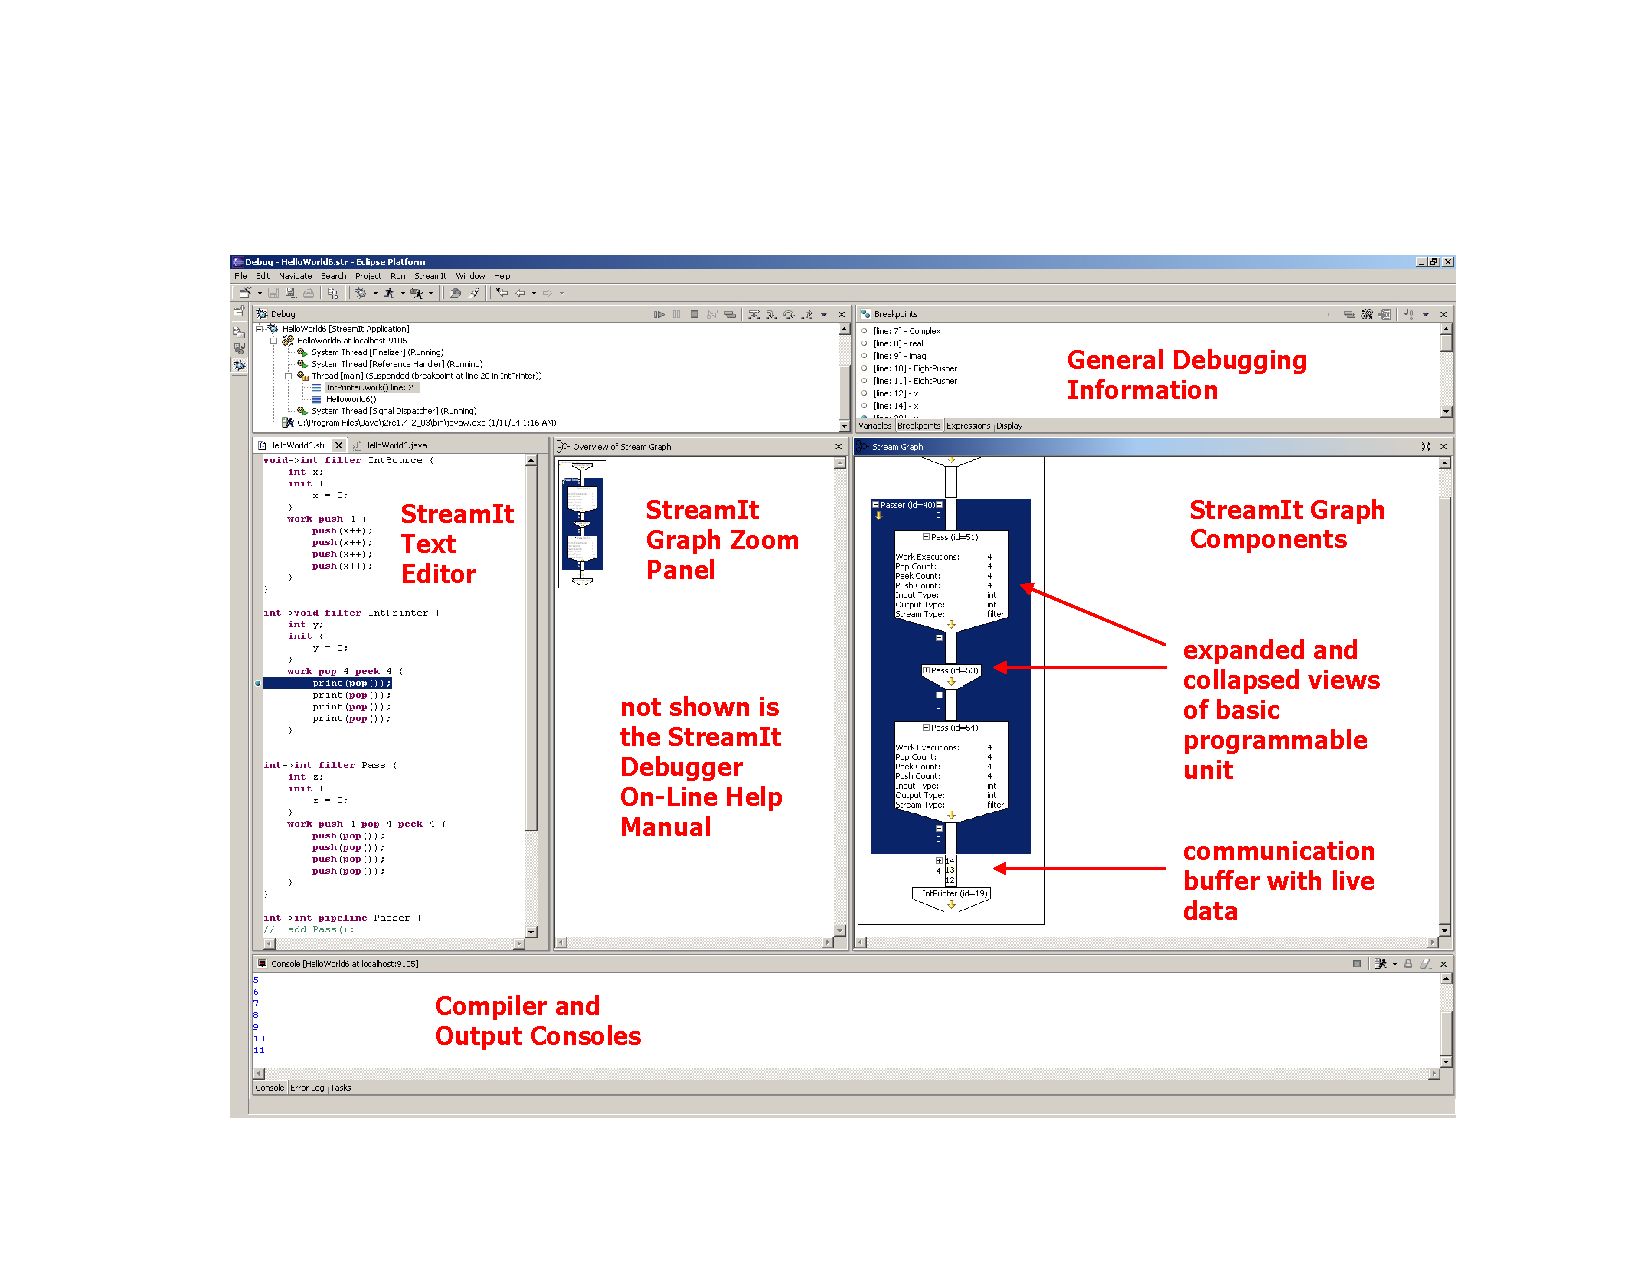
\includegraphics[width=3.0in, angle=270]{kuo_figure1.pdf}}
  \caption{A screen-shot of the StreamIt debugger.} 
  \label{kuo_figure1}
\end{figure}

\absection{Progress}

We  have recently  made  available  the first  public  version of  the
StreamIt Development Tool (SDT).  It  is implemented in Java as a {\it
plug-in}  extension  to   Eclipse---a  universal  platform  for  tools
integration  (see {\it www.eclipse.org}  for more  information on Eclipse).
The SDT  is a  graphical programming environment,  and it  consists of
several  components that  enable the  development,  visualization, and
debugging  of programs  written in  StreamIt.  The  SDT  debugger (see
Figure~\ref{kuo_figure1} for a  screen-shot) can interpret and visually
represent  the stream graph  and its  dynamic behavior,  including the
flow of  information in parallel  streaming components.  The  SDT also
includes a tutorial and extensive documentation.

\absection{Future}

There are  two main directions that  we hope to explore  in our future
work.  First,  we  would  like  to  formally evaluate  the  SDT  as  a
productivity  tool.   That  is,  to  what extent  does  the  graphical
development and  debugging environment help  programmers implement and
verify  the correctness  of StreamIt  applications?  We  are currently
evaluating  various  options  for   conducting  a  set  of  controlled
experiments  to   explicitly  quantify  the  SDT   impact  on  overall
programmer productivity; we believe the advantages afforded by the SDT
are significant when compared to conventional methodologies.
Second, we plan to thoroughly  evaluate the scalability of the SDT for
massively  parallel  applications,   with  thousands  of  filters  and
communication  edges.   In  particular,   we  would  like  to  explore
different  scenarios  for visualizing  and  debugging highly  parallel
stream graphs.

%% This section is the one of the most important ones.  Please check 
%% with your research supervisor to make sure all the relevant funding
%% agencies for your project are acknowledged.

\absection{Research Support}
This work is supported in part by a grant from DARPA (PCA
F29601-04-2-0166), awards from NSF (CISE EIA-0071841, ITR ACI-0325297,
NGS CNS-0305453), and a fellowship from the MIT-Oxygen Project.

%% The abstract bibliographies should be done using bibtex.  Please
%% compile your bibtex entries into a single file with a distinguishing
%% name. The \absbibliography command is analogous to the \bibliography
%% command, taking a single argument, the name of your bibtex file, 
%% minus the .bib extention. The \bibliographystyle command should not
%% be used.  You can use a single bibliography file if you are submitting
%% multiple abstracts.  

\absbibliography{kuo_bib}

\end{document}
